\documentclass[10pt]{article}
\usepackage{icmlko}

\icmlmeta{IP 파운데이션 월드모델}{177}{어렵게 찾은 것이 더 유명했다}{노트 176이 ``새로 찾은 문서는 조회수가 제일 낮을 것''이라 가정하고 시뮬레이션했다. 실제로 재 보니 반대였고, 결론의 부호는 살아남았지만 크기가 다섯 배 줄었다}

\begin{document}

\twocolumn[
\icmlheader

\begin{abstract}
노트 176이 ``빈칸을 채우면 판이 내려간다''를 보이면서 새로 채운 레코드에
관측 \emph{최저값} 을 줬고, 그 가정을 검정 안 했다고 적었다. 검정할 자료가
있다 --- 위키 수집 캐시에 매칭 방식이 남아 있다. 제목을 바로 대서 찾은
것(\texttt{직접})과 되돌리기 사슬을 타야 찾은 것(\texttt{검색} ·
\texttt{프랜차이즈} · \texttt{맨제목})을 견주면 ``찾기 어려웠던 레코드''의
성격을 알 수 있다. \textbf{가정이 반대였다.} 어렵게 찾은 1,055건의 $\log$
조회수 중앙이 \textbf{5.45} 이고 쉽게 찾은 1,391건은 \textbf{5.05} 다
($p{=}1.4\times10^{-13}$). 특히 프랜차이즈 되돌리기로 찾은 165건이
\textbf{6.41} 로 제일 높다 --- 속편이라 자기 문서가 없었던 대형 IP 들이다.
그래서 시뮬레이션을 네 규칙으로 다시 했다. \textbf{모든 규칙에서 판이
내려가지만 크기가 다르다} --- 최저값 $-$0.040(노트 176), 관측 분포
$-$0.028, 상위 절반 $-$0.019, 중앙값 $-$0.008. \textbf{노트 176의 ``위키
이득의 네 배''는 최악의 경우였고 현실적인 규칙에서는 두세 배다.} 그리고
\textbf{``능형은 거의 안 움직인다''는 틀렸다} --- 최저값 규칙에서만
$-$0.001이었고 관측 분포에서는 $-$0.018로 배깅($-$0.028)과 비슷하다.
마지막으로 하나 더 나왔다. \textbf{채울 수 있는 모집단이 애초에 작다} ---
유보에서 위키 문서를 아예 못 찾은 비율이 도서 · 펀딩 · 아이돌
\textbf{100\%}, 웹툰 92\%, 모바일 93\%다. 그 도메인들은 위키 축이 처음부터
없는 것과 같고, 마스크 신호가 사는 곳은 게임(61\%) · 애니(60\%) ·
팝업(46\%) · 세계애니(8\%) 넷뿐이다.
\end{abstract}
]

\begin{figure*}[t]
\centering
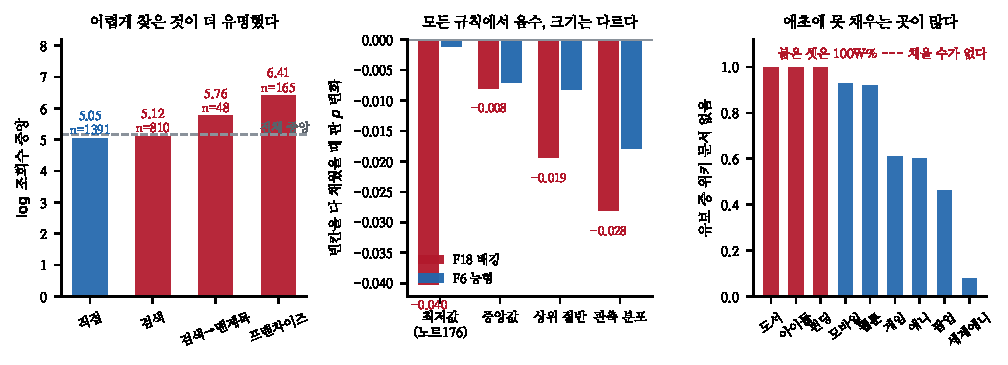
\includegraphics[width=\textwidth]{figs/assume.pdf}
\caption{왼쪽 --- 어렵게 찾은 것이 더 유명했다. 가운데 --- 모든 규칙에서
음수, 크기는 다르다. 오른쪽 --- 애초에 못 채우는 곳이 많다.}
\end{figure*}

\section{가정이 반대였다}

\begin{table}[t]
\centering\tsize
\caption{매칭 방식별 $\log$ 조회수. 2,446건.}
\begin{tabular}{lrr}
\toprule
& n & 중앙 \\
\midrule
직접 (쉬움) & 1{,}391 & \textbf{5.05} \\
검색 & 810 & 5.12 \\
검색→맨제목 & 48 & 5.76 \\
\textbf{프랜차이즈} & 165 & \textbf{6.41} \\
\midrule
어려운 매칭 전체 & 1{,}055 & \textbf{5.45} \\
\bottomrule
\end{tabular}
\end{table}

\claimx{\textbf{어렵게 찾은 것이 더 유명했다}($p{=}1.4\times10^{-13}$).
노트 176이 반대로 가정했다.}{까닭이 보인다 --- 프랜차이즈 되돌리기는
``$\cdots$ season 3'' 같은 속편에서 걸리고, 속편은 자기 문서가 없을 뿐
프랜차이즈가 크다. \textbf{매칭 난이도는 저명성이 아니라 제목의 모양을
잰다.}}

\claimx{\textbf{다만 완전한 대리는 아니다.} ``어렵게 찾았지만 찾은''
레코드와 ``끝내 못 찾은'' 레코드는 다르다. 후자는 진짜로 문서가 없는
쪽에 가깝다.}{그러니 실제 채움의 값 분포는 이 둘 사이 어디일 것이다 ---
그래서 네 규칙을 다 재 봤다.}

\section{네 규칙으로 다시}

\begin{table}[t]
\centering\tsize
\caption{유보 빈칸을 100\% 채웠을 때 판 $\rho$ 변화.}
\begin{tabular}{lrr}
\toprule
채움 값 & F18 배깅 & F6 능형 \\
\midrule
최저값 (노트 176) & \textbf{$-$.0402} & $-$.0011 \\
관측 분포에서 뽑음 & $-$.0281 & \textbf{$-$.0179} \\
상위 절반에서 뽑음 & $-$.0194 & $-$.0081 \\
중앙값 & $-$.0080 & $-$.0071 \\
\midrule
(위키 축 전체 이득) & $+$.0096 & $+$.0138 \\
\bottomrule
\end{tabular}
\end{table}

\claimx{\textbf{부호는 살아남고 크기가 준다.} 네 규칙 전부 음수이므로
``채우면 판이 내려간다''는 결론은 유지된다. 다만 노트 176의 $-$0.040은
최악의 경우이고 현실적인 규칙에서는 $-$0.008$\sim$$-$0.028이다.}{``위키
이득의 네 배''를 ``한 배에서 세 배''로 고친다.}

\claimx{\textbf{``능형은 거의 안 움직인다''는 틀렸다.} 최저값 규칙에서만
$-$0.001이었고 관측 분포에서는 $-$0.018로 배깅($-$0.028)과 비슷하다.}{노트
176이 그것을 ``트리가 더 많이 쓰고 더 쉽게 배신당한다''의 다섯 번째
사례로 셌는데, \textbf{그 사례는 취소한다.} 앞의 네 개(노트 156 · 161 ·
171 · 174)는 그대로다.}

\section{애초에 못 채우는 곳이 많다}

\begin{table}[t]
\centering\tsize
\caption{유보 레코드 중 위키 문서를 아예 못 찾은 비율.}
\begin{tabular}{lr}
\toprule
\textbf{도서 · 펀딩 · 아이돌} & \textbf{100\%} \\
모바일 & 93\% \\
웹툰 & 92\% \\
게임 & 61\% \\
애니 & 60\% \\
팝업 & 46\% \\
세계애니 & 8\% \\
\bottomrule
\end{tabular}
\end{table}

\claimx{\textbf{세 도메인은 유보 전체가 문서 없음이다.} 도서 · 펀딩 ·
아이돌에서 위키 축은 처음부터 없는 것과 같다. 마스크 신호가 사는 곳은
게임 · 애니 · 팝업 · 세계애니 넷뿐이다.}{그러니 ``수집을 개선하면''이라는
시나리오 자체가 그 넷에만 해당한다. 노트 176이 전 도메인 이야기처럼
적었는데 그렇지 않다.}

\claimx{\textbf{그리고 그 빈칸은 대개 못 채운다.} 노트 150에서 직접 →
프랜차이즈 → 검색(겹침 검사)까지 되돌리기 사슬을 다 돌린 뒤 남은 것들이다.
\textbf{남은 빈칸은 진짜로 문서가 없는 IP 다.}}{한국어 위키를 더 대거나
다른 언어판을 붙이면 조금 더 찾을 수 있다 --- 노트 158에서 팝업에
한국어판을 붙여 60\%를 얻은 것이 그 예다.}

\section{그래서 노트 176을 어떻게 읽나}

\begin{table}[t]
\centering\tsize
\caption{노트 176의 주장과 이 노트의 정정.}
\begin{tabular}{ll}
\toprule
살아남음 & 빈칸을 채우면 판이 내려간다 \\
살아남음 & 마스크는 참 신호다($t{=}2.3$ · $3.4$) \\
살아남음 & 판 $\rho$ 가 수집 불완전성도 잰다 \\
\midrule
\textbf{고침} & 네 배 $\to$ 한 배$\sim$세 배 \\
\textbf{취소} & ``능형은 안 움직인다'' \\
\textbf{좁힘} & 네 도메인 이야기다 \\
\bottomrule
\end{tabular}
\end{table}

\begin{table}[t]
\centering\tsize
\caption{남은 것.}
\begin{tabular}{ll}
\toprule
\textbf{언어판} & 도서 · 펀딩 · 아이돌은 한국어판을 안 대 봤다 \\
값 분포 & 실제로 새로 찾아서 재는 것이 제일 정확하다 \\
매칭 난이도 & 제목 모양의 대리일 뿐 --- 자질로 쓰면 안 된다 \\
\bottomrule
\end{tabular}
\end{table}

첫 줄이 곧바로 할 수 있는 일이다. 도서 · 펀딩 · 아이돌은 영문 위키만 대
봤고 한국어판은 안 댔다. \textbf{노트 158에서 팝업이 한국어판으로 60\%를
얻었으니 이 셋도 0\%는 아닐 것이다} --- 그리고 그러면 시뮬레이션이 아니라
실측으로 이 노트의 질문에 답할 수 있다.

\end{document}
